\documentclass[10pt]{article}
\usepackage{icmlko}

\icmlmeta{IP 파운데이션 월드모델}{64}{진단 코드가 세 번 거짓말했다}{본 파이프라인은 규약을 지키는데 그것을 검사하려고 급히 쓴 코드가 안 지켰다 --- 세 노트에서 같은 일이 났다}

\begin{document}

\twocolumn[
\icmlheader

\begin{abstract}
노트 63이 남긴 항목 둘을 처리하다가 패턴을 발견했다. 첫째, ``원본을 못 찾은
7건''은 다른 디렉터리에 있었다 --- 시장 레코드다. \textbf{미매칭은 0건이다.}
둘째, 노트 52가 ``아이돌 소속사 정규화가 빠져 있다''고 지적한 것을 고치려고
본 코드를 열었더니 \texttt{norm\_agency}가 \textbf{이미 있었다} --- `SM
Entertainment' / `SM 엔터테인먼트' / `SM'을 하나로 묶는다. 정규화가 빠져 있던
것은 파이프라인이 아니라 노트 52를 쓸 때 급히 짠 진단 코드였다. 그러고 보니
노트 54에서도 같은 일이 있었다 --- 게임 고유 축의 짝지은 구간이
{[}$-$0.167, $-$0.027{]}로 나와 ``해롭다''고 읽을 뻔했는데, 원인은 복원추출
\emph{뒤에} 고유 축을 붙여 레코드 대응이 깨진 것이었다. 고치니
{[}$+$0.001, $+$0.011{]}로 부호가 뒤집혔다. \textbf{세 번 다 본 파이프라인은
옳았고 진단 코드가 틀렸다.} 공통 원인이 하나다 --- 진단을 급히 짜면서 본 코드가
지키는 규약(이름 정규화 · 레코드 대응 · 데이터 경로)을 재현하지 않았다.
처방은 단순하다. \textbf{진단은 본 코드의 함수를 불러 쓴다.} 부수로 확인한 것도
있다. 정규화하면 아이돌 소속사가 68개에서 54개로 줄고 2건 이상이 5개에서 13개로
느는데, 이력 보유 레코드는 여전히 17/81이라 \textbf{노트 52의 ``표본 부족''
결론 자체는 유지된다}.
\end{abstract}
]

\section{두 항목을 처리하다가}

\paragraph{미매칭 7건}
노트 63은 분석 풀 75건 중 68건만 원본을 찾았다고 적었다. 디렉터리를 넓혀
다시 찾으니 나머지 7건은 \texttt{data/market\_records}에 있었다 --- 내부 팝업이
아니라 외부 보도 기반 시장 레코드다. \textbf{미매칭은 0건이다.} 노트 63의
한계 항목 첫 줄을 지운다.

\paragraph{소속사 정규화}
노트 52는 이렇게 적었다 --- ```SM'과 `SM엔터테인먼트'가 따로 세어진다.
정규화가 빠져 있다.'' 고치려고 \texttt{ingest/idol\_axes.py}를 열었더니 이미
있었다.

\begin{quote}\fontsize{9.5}{11.5}\selectfont
\texttt{norm\_agency} --- ``\,`SM Entertainment' / `SM 엔터테인먼트' / `SM'을
하나로 묶는다. 정규화 전 205개 고유값 중 상당수가 같은 회사의 표기 차이였다.''
\end{quote}

정규화가 빠져 있던 것은 노트 52를 쓸 때 급히 짠 진단 코드였다.

\section{세 번째다}

\begin{figure}[t]
\centering
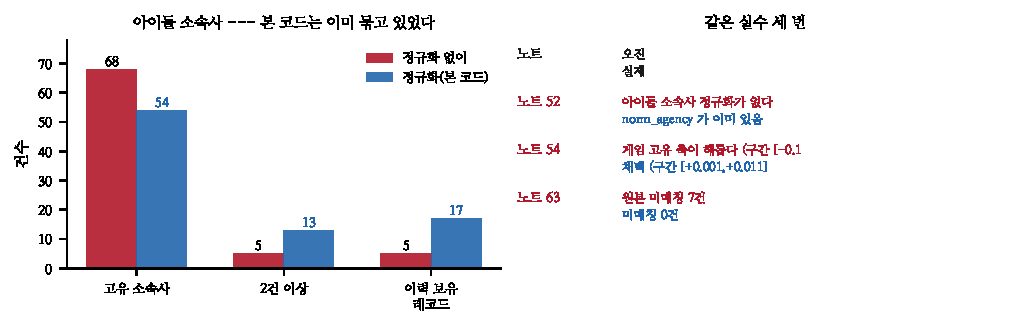
\includegraphics[width=\textwidth]{figs/diaglies.pdf}
\caption{왼쪽 --- 아이돌 소속사. 오른쪽 --- 세 오진.}
\end{figure}

\begin{table}[t]
\centering\tsize
\caption{진단 코드가 만든 오진.}
\begin{tabular}{lll}
\toprule
노트 & 오진 & 실제 \\
\midrule
52 & 정규화가 없다 & 있었다 \\
54 & 고유 축이 해롭다 & 이롭다(부호 반전) \\
63 & 미매칭 7건 & 0건 \\
\bottomrule
\end{tabular}
\end{table}

노트 54가 가장 심했다. 게임 고유 축의 짝지은 구간이 $[-0.167,\ -0.027]$로
나와 점추정($+$0.0066)과 정반대였다. 원인은 복원추출 \emph{뒤에} 고유 축을
붙여 원본 순서의 축이 재추출된 행에 걸린 것이다. 길이가 맞아 오류도 안 났다.
고치니 $[+0.001,\ +0.011]$로 채택이 됐다.

\claimx{세 번 다 본 파이프라인은 옳았고 진단 코드가 틀렸다. 공통 원인은 진단을
급히 짜면서 본 코드가 지키는 규약 --- 이름 정규화, 레코드 대응, 데이터 경로 ---
을 재현하지 않은 것이다.}{네 번째가 나오면 규율로는 안 되는 것이고 구조로 막아야
한다. 지금은 ``진단은 본 코드의 함수를 불러 쓴다''는 규칙만 세운다.}

\paragraph{왜 하필 진단 코드인가}
본 코드는 노트를 쓸 때마다 검정을 통과해야 하고 다음 노트에서 다시 쓰인다.
진단 코드는 한 번 쓰고 버린다. 그래서 규약이 안 실린다. 그런데 \textbf{판정을
내리는 것은 진단 코드다} --- 본 코드는 값을 만들고 진단 코드가 그 값을 해석한다.
검증이 가장 약한 자리에서 결론이 나온다.

\section{정규화 결과는 결론을 안 바꾼다}

\begin{table}[t]
\centering\tsize
\caption{아이돌 소속사. 표본 81건.}
\begin{tabular}{lrr}
\toprule
& 정규화 없이 & 정규화 \\
\midrule
고유 소속사 & 68개 & 54개 \\
2건 이상 & 5개 & \textbf{13개} \\
사전 이력 보유 레코드 & 5건 & \textbf{17건} \\
\bottomrule
\end{tabular}
\end{table}

2건 이상 소속사가 두 배 반이 되고 이력 보유가 세 배가 된다. 그래도 17/81이라
상관을 재기에 부족하다(문턱 25건). \textbf{노트 52의 ``아이돌은 표본 부족으로
못 잰다''는 유지된다} --- 이유가 정확해졌을 뿐이다. 정규화를 안 해서가 아니라
81건에 소속사가 54개라서다.

\section{한계}

\begin{itemize}[leftmargin=1.1em,itemsep=0.15em]
\item 세 사례를 모아 패턴이라 했지만 노트 예순넷 중 셋이다. 진단 코드를 쓴
      횟수로 나누면 비율은 모른다.
\item ``진단은 본 코드의 함수를 불러 쓴다''를 규칙으로만 세웠고 강제하지 않았다.
\item 앞선 노트들의 진단 코드를 전수 재검토하지 않았다. 같은 종류의 오진이
      더 있을 수 있다.
\item 아이돌 이력을 정규화해서 다시 쟀지만 17건이라 상관을 못 냈다. 문턱을
      낮추면 재겠지만 그 자체가 자의적이다.
\item 노트 63의 ``7건 미매칭''을 지웠는데, 그 7건이 시장 레코드라 등급 체계가
      다르다. 노트 63의 등급 분포(A 53 · B 15)는 68건 기준이다.
\end{itemize}

\section{다음}

\begin{enumerate}[leftmargin=1.3em,itemsep=0.15em]
\item 앞선 노트들의 진단 코드를 훑어 같은 오진이 더 있는지 본다.
\item 시장 레코드 7건의 라벨 신뢰를 따로 매긴다.
\item 웹툰 전체 수집 완료 후 전면 재측정(2,006/3,973 진행 중).
\item 진단에 쓸 공용 함수를 모듈로 뽑는다 --- 규칙보다 구조가 낫다.
\end{enumerate}

\vspace{0.6em}
\hrule height 0.3pt
\vspace{0.5em}
{\footnotesize
\textbf{참고문헌}\\[0.3em]
Hoare, C. A. R. (1981). The emperor's old clothes. \emph{CACM}, 24(2), 75--83.\\[0.15em]
Northcutt, C. G., Athalye, A., Mueller, J. (2021). Pervasive label errors in test
sets. \emph{NeurIPS D\&B}.\\[0.15em]
Efron, B., Tibshirani, R. J. (1993). \emph{An Introduction to the Bootstrap}.
Chapman \& Hall.\\[0.15em]
Bouthillier, X. et al. (2021). Accounting for variance in machine learning
benchmarks. \emph{MLSys}, 3, 747--769.\\[0.15em]
Ben-David, S. et al. (2010). A theory of learning from different domains.
\emph{Machine Learning}, 79(1--2), 151--175.
}

\end{document}
